% Use Roman numerals (i, ii, iii, etc.) for page numbers in the front matter.
\pagenumbering{roman}

%%%%%%%%%%%%%%%%%%%%%%%%%%%%%%%%%%%%%%%%%%%%%%%%%%%%%%%%%%%%%%%%%
%% TITLE PAGE.
%%%%%%%%%%%%%%%%%%%%%%%%%%%%%%%%%%%%%%%%%%%%%%%%%%%%%%%%%%%%%%%%%

% No headers or footers on the title page.
\thispagestyle{empty}

\begingroup
\centering
\setstretch{1.0}
~
\\[1em]
\sffamily\bfseries\fontsize{26}{31.2}\selectfont
\DocumentTitle
\\
Use Manual Line Breaks If Necessary
\\[0.4in]
\normalfont\large
Thesis by
\\[0.25em]
\sffamily\bfseries\Large
\AuthorName
\\[0.4in]
\normalfont\normalsize
In Partial Fulfillment of the Requirements
\\[0.5em]
for the Degree of
\\[0.5em]
Doctor of Philosophy
\\[0.5em]
in
\\[0.5em]
Electrical Engineering and Computer Science
\vfill
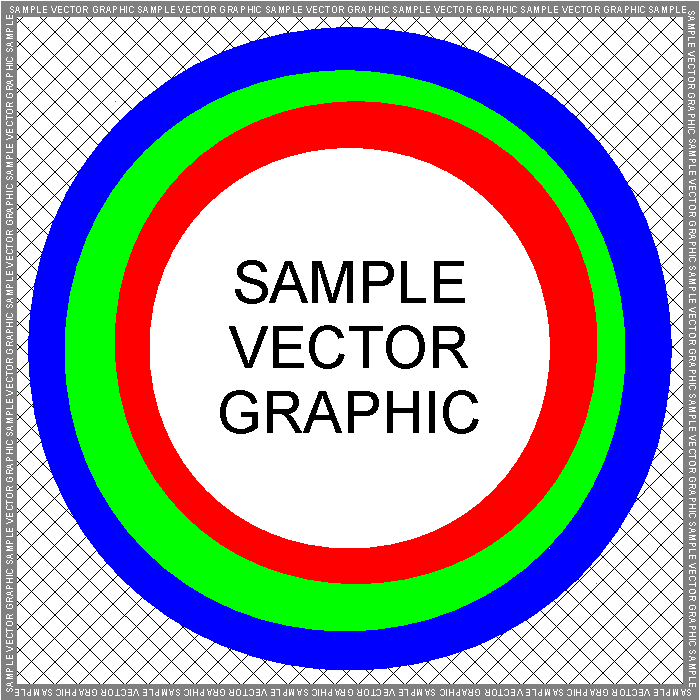
\includegraphics[height=1.8in]
{Figures/Figure-SchoolLogo}
\\[1.5em]
University Institute of College
\\[0.5em]
Springfield, New York, USA
\\[1.5em]
2016
\\[0.5em]
(Defended November 25, 2016)
\par
\endgroup

\clearpage
